\begin{blocksection}
\question Draw the box-and-pointer diagram. \\

\begin{lstlisting}
>>> violet = [7, 77, 17]
>>> violet.append([violet.pop(1)])

>>> dash = violet * 2
>>> jack = dash[3:5]
>>> jackjack = jack.extend(jack)

>>> helen = list(violet)
>>> helen += [jackjack]
>>> helen[2].append(violet)
\end{lstlisting}

\begin{solution}[1in]
\url{https://goo.gl/EAmZBW}

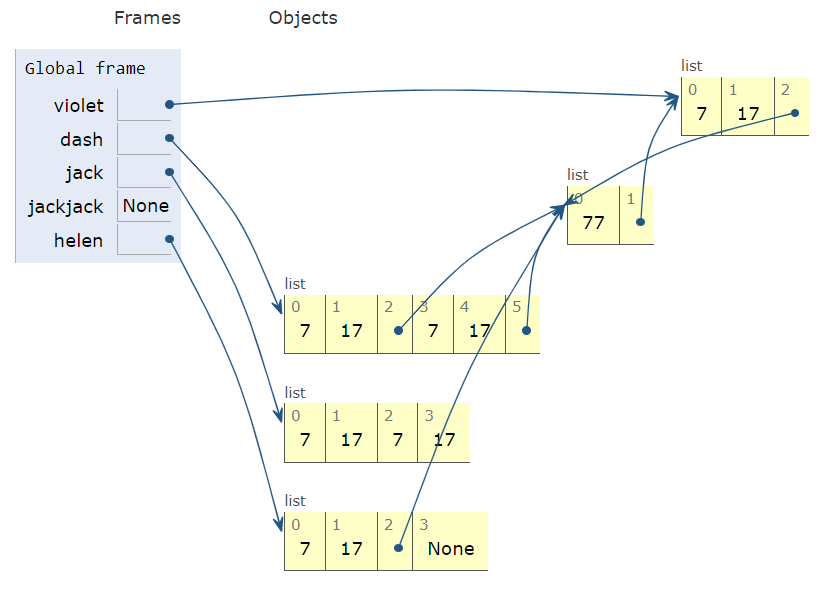
\includegraphics[width=0.8\textwidth]{incredibles.png}
\end{solution}
\end{blocksection}

\begin{guide}
    \textbf{Teaching Tips}
    \begin{itemize}
       \item Draw out the box and pointer diagram for each part.
       \item Try to highlight when pointers change vs. when the values a pointer points to change.
       \item If students are very confused about this problem, try going over the PythonTutor!
    \end{itemize}
 \end{guide}
